\documentclass[conference]{IEEEtran}
\IEEEoverridecommandlockouts

\usepackage{cite}
\usepackage{amsmath,amssymb,amsfonts}
\usepackage{booktabs}
\usepackage{array}
\usepackage{graphicx}
\usepackage{tikz}
\usetikzlibrary{arrows.meta,positioning}
\usepackage{xcolor}
\usepackage{url}
\usepackage{balance}
\usepackage{flafter}

\begin{document}

\title{Lumina: Confidence-Weighted Identity Fusion\\ and Preference-Aware Ranking for Photo Curation}

\author{
\IEEEauthorblockN{Agustinus Benyamin Prasetyo and Ong Qing Quan}
\IEEEauthorblockA{Institute of Systems Science, National University of Singapore\\
Singapore 119615\\
Capstone Group 10}
}

\maketitle

\begin{abstract}
Lumina curates a personal photo batch into events and people, then selects a
best shot of each person at each event. The Semester~1 prototype already
combined face embeddings, body re-identification, scene embeddings and a
weighted aesthetic ranker, but identity was not fused, event boundaries
depended on who appeared in the frame, and the ranker could not express a
blink, a near-duplicate burst, or a user's taste. This paper specifies the
capstone model. Faces are matched to person boxes by a one-to-one assignment
with a head-position prior. ArcFace and OSNet embeddings are placed in separate
blocks of a concatenated vector, scaled by a confidence weight $\alpha\in[0.7,1]$,
so that cosine similarity in the fused space is an $\alpha$-weighted blend of
the two modalities. Events are agglomerative clusters on \mbox{DINOv3} distances
blended with capture time, named by CLIP against a closed prompt bank.
Ranking uses seven signals with floored normalisation, an absolute eyes-open
score, and a hard constraint that a detected blink loses to any eyes-open
alternative. A Bradley--Terry update turns a user's swap into one gradient step
on the weight vector. On a private set of 55 photographs in 20 occasions, the
label-free event threshold reaches an adjusted Rand index of $0.985$ against
the folder grouping, against $0.549$ for the Semester~1 event features, and
identity clustering makes none of the 526 merges that would put two faces from
one photograph in the same person. Thirteen people choosing which frame to keep
score the displayed order at $0.53$ against $0.50$ for a random pick: above
chance, and too small a margin to keep only one frame or to delete another
without a stated reason. Preferences vary, within and across people. On one
occasion every tester kept the frame that shows the whole party, which the
ranker had placed last. One preference pass does not raise held-out agreement.
\end{abstract}

\begin{IEEEkeywords}
photo curation, face recognition, person re-identification, event clustering,
learning to rank, preference learning
\end{IEEEkeywords}

\section{Introduction}
\label{sec:intro}

A holiday, a wedding or a family weekend produces a pile of near-duplicate
photographs. The useful output is not another grid of files. It is a small set
of events, a cast of people, and one defensible shot of each person in each
event. That task has three coupled decisions: who is the same person when the
face is small, turned or missing; which photographs belong to the same
occasion when the background barely changes; and which frame is the one to
keep when several are acceptable.

Phone galleries cluster faces. They do not rank a burst, explain the choice,
or change that choice when the user prefers another frame. Lumina composes
published encoders and puts the modelling effort into the fusion, the
clustering objective, the constraints on the ranker, and a preference update
from a handful of pairwise edits.

The Semester~1 baseline detected people with YOLOv8~\cite{jocher2023yolov8},
embedded bodies with OSNet~\cite{zhou2019osnet}, clustered them with
HDBSCAN~\cite{mcinnes2017hdbscan}, embedded scenes with a DINO-family
model, scored aesthetics with NIMA~\cite{talebi2018nima}, and ranked each
event with seven hand-set weights. Its own measurements, on a few dozen
photographs, already pointed at the next model rather than at more of the same
pipeline. HDBSCAN's silhouette on re-identification embeddings was about
$0.25$, against about $0.79$ for a tuned DBSCAN. Adding a person
co-attendance block to the event features raised silhouette only from $0.764$
to $0.775$. An ablation of the ranker found that the eye-aspect term never
changed a winner, which is evidence that the term had no usable dynamic range,
not evidence that blinks are unimportant.

This paper treats those findings as the problem statement. The contributions
are:
\begin{enumerate}
\item a confidence-weighted concatenation of ArcFace~\cite{deng2019arcface}
and OSNet that keeps cosine similarity equal to a modality blend, with a floor
on the face weight so that a face with a body and the same face without one
still meet;
\item event clustering on time-blended \mbox{DINOv3} distances, dropping identity
from the event features so that a clustering error about people cannot define
the occasion;
\item a ranker whose normalisation, eyes-open score and blink constraint are
specified so that burst noise and closed eyes cannot win on a rescaled
aesthetic gap;
\item an online Bradley--Terry update~\cite{bradley1952rank} of the seven
weights, with the operating step scored by asking people which photograph they
would keep;
\item an identity check, using the same ArcFace model, that discards a
generative retouch when the weakest face match falls below a set cosine.
\end{enumerate}
Items 1--4 are what Section~\ref{sec:eval} measures. Naming, search, captions
and retouching (Section~\ref{sec:support}) read that output and do not change
it. There is no public-album benchmark.

\section{Related work}
\label{sec:related}

Time has been an event feature since PhotoTOC, which clustered photographs by
creation time and colour~\cite{platt2003phototoc}. Later galleries replaced
colour with learned scene descriptors and added a separate face
clustering. Lumina keeps that split and adds a ranker between them.

ArcFace embeddings are compared by cosine~\cite{deng2019arcface}; the detector
and the 512-dimensional face vector are InsightFace
\texttt{buffalo\_l}~\cite{insightface}. OSNet supplies a 512-dimensional body
vector when the face is missing~\cite{zhou2019osnet}, from YOLOv8
boxes~\cite{jocher2023yolov8}. The two vectors are not one space, so they are
concatenated rather than averaged. HDBSCAN fits a density that has no known
threshold~\cite{mcinnes2017hdbscan}; a face embedding trained for a cosine
cutoff does not. Scene descriptors are \mbox{DINOv3}, with DINOv2 as a
fallback~\cite{oquab2024dinov2,simeoni2025dinov3}. CLIP names an event from a
fixed prompt list~\cite{radford2021clip}. BLIP captions the selected frame
only~\cite{li2022blip}. NIMA contributes one aesthetic term, not the
rank~\cite{talebi2018nima,murray2012ava}. MMR trades that score against
redundancy when the output is a set~\cite{carbonell1998mmr}. Bradley--Terry
updates the weights from a pairwise swap~\cite{bradley1952rank}. Silhouette
picks the event threshold and is not a substitute for a
label~\cite{rousseeuw1987silhouettes}.

\section{Model}
\label{sec:model}

A job is a set of images $\{I_i\}_{i=1}^{N}$, $N$ up to a few hundred. Each
image may carry an EXIF capture time $t_i$. The model returns a partition of
images into events, a set of identity clusters, a total order inside each
event, a best photograph per person inside each event, three highlight sets,
optional text-query ranks, and a weight vector that later jobs can reuse.
The application shows events as \emph{moments}.
Figure~\ref{fig:pipeline} is the data flow. Encoders are frozen. Everything
after the embeddings is deterministic given the configuration in
Table~\ref{tab:operating}. Association, fusion, events, the ranker and
preference learning decide the curation. Naming, search, captions and
retouching do not feed back into it.

\begin{figure}[t]
\centering
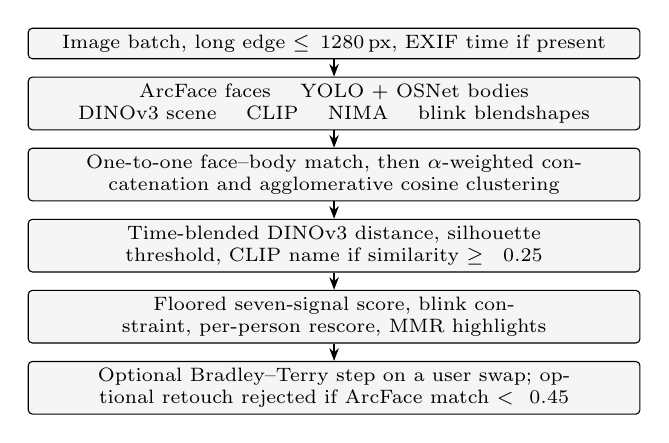
\begin{tikzpicture}[
  font=\scriptsize,
  node distance=2.2mm,
  box/.style={draw, rounded corners=1.5pt, align=center,
              inner sep=2.4pt, fill=black!4, text width=7.6cm},
  arr/.style={-{Stealth[length=1.6mm]}, semithick}
]
\node[box] (in) {Image batch, long edge $\le 1280$\,px, EXIF time if present};
\node[box, below=of in] (enc) {ArcFace faces \quad YOLO + OSNet bodies\\
\mbox{DINOv3} scene \quad CLIP \quad NIMA \quad blink blendshapes};
\node[box, below=of enc] (id) {One-to-one face--body match, then
$\alpha$-weighted concatenation and agglomerative cosine clustering};
\node[box, below=of id] (ev) {Time-blended \mbox{DINOv3} distance, silhouette threshold,
CLIP name if similarity $\ge 0.25$};
\node[box, below=of ev] (rk) {Floored seven-signal score, blink constraint,
per-person rescore, MMR highlights};
\node[box, below=of rk] (out) {Optional Bradley--Terry step on a user swap;
optional retouch rejected if ArcFace match $<0.45$};
\draw[arr] (in) -- (enc);
\draw[arr] (enc) -- (id);
\draw[arr] (id) -- (ev);
\draw[arr] (ev) -- (rk);
\draw[arr] (rk) -- (out);
\end{tikzpicture}
\caption{Capstone inference path. Encoders are pretrained and frozen. Identity
and events are separate partitions. Preference learning and retouching run
only when the user asks.}
\label{fig:pipeline}
\end{figure}

\begin{table}[t]
\caption{Operating points used by the capstone model.}
\label{tab:operating}
\centering
\scriptsize
\begin{tabular}{@{}>{\raggedright\arraybackslash}p{3.05cm}>{\raggedright\arraybackslash}p{4.55cm}@{}}
\toprule
Choice & Value \\
\midrule
Face embedding & InsightFace \texttt{buffalo\_l}, 512-d \\
Body embedding & OSNet-x1.0, $256\times128$, 512-d \\
Scene embedding & \mbox{DINOv3} ViT-S/16 (DINOv2-base fallback) \\
Text--image & CLIP ViT-B/32 \\
Aesthetic & NIMA (AVA), one scalar in $[0,10]$ \\
Face cluster distance & $0.60$ cosine (face-only ablation) \\
Fused cluster distance & $0.58$ cosine \\
Body attach distance & $0.75$ Euclidean to ReID centroid \\
$\alpha$ range & $[0.7,\,1.0]$ \\
Event time weight, $\tau$ & $0.35$,\ $6$ hours \\
Event threshold sweep & $[0.05,1.0)$ step $0.025$, patience $10$ \\
Duplicate cosine & $\ge 0.965$ on \mbox{DINOv3} \\
Blink reject & eyes-open $< 0.45$ and a face was detected \\
MMR $\lambda$ & $0.90$ / $0.70$ / $0.45$ (at most 6) \\
Preference step, prior pull & $\eta=0.20$,\ $\lambda_{\mathrm{prior}}=0.05$ \\
Retouch reject / warn & ArcFace cosine $0.45$ / $0.65$ \\
\bottomrule
\end{tabular}
\end{table}

\subsection{Associating a face with a body}
\label{sec:assoc}

Semester~1 linked a face to the first person box that contained it. Overlapping
people in a group photograph then shared a face. The replacement is a greedy
one-to-one assignment. For face box $f$ and person box $p$, let $c(f,p)$ be
the fraction of the face area inside the person box. Pairs with
$c(f,p)<0.5$ are discarded. Among the rest the score is
\begin{equation}
c(f,p) + 0.5\, h(f,p),
\label{eq:match}
\end{equation}
where the head prior $h$ is high when the face centre is near the horizontal
centre of the person box and in its upper portion. With person width $w$ and
height $h_p$, and face centre $(x,y)$,
\begin{equation}
h = \max(0, 1-\Delta x)\,
    \max\!\left(0,\; 1-\min(\Delta y/0.6,\, 1)\right),
\end{equation}
$\Delta x = |x - \bar{x}_p|/w$ and $\Delta y = (y - y^{\mathrm{top}}_p)/h_p$.
Candidates are taken in descending score. Each face and each person box is used
at most once. A body with no assigned face, and a face with no assigned body,
both remain in the pipeline; fusion treats the missing block as empty rather
than imputing it.

\subsection{Confidence-weighted embedding fusion}
\label{sec:fusion}

Let $\hat{f}$ and $\hat{b}$ be L2-normalised ArcFace and OSNet vectors. They
are not added. The fused descriptor is the concatenation
\begin{equation}
u =
\begin{bmatrix}
\sqrt{\alpha}\,\hat{f}\\[2pt]
\sqrt{1-\alpha}\,\hat{b}
\end{bmatrix},
\label{eq:fuse}
\end{equation}
which already has unit norm when both blocks are present. For two detections
with weights $\alpha_i$ and $\alpha_j$,
\begin{equation}
u_i^{\mathsf T} u_j
=
\sqrt{\alpha_i\alpha_j}\;
\hat{f}_i^{\mathsf T}\hat{f}_j
+
\sqrt{(1-\alpha_i)(1-\alpha_j)}\;
\hat{b}_i^{\mathsf T}\hat{b}_j.
\label{eq:cos}
\end{equation}
When $\alpha_i=\alpha_j=\alpha$ this is exactly
$\alpha$ times the face cosine plus $(1-\alpha)$ times the body cosine. A
missing modality forces $\alpha$ to $1$ (face only) or $0$ (body only) and
zeros the other block, so similarity falls back to the modality the two
detections share.

The weight itself is a detection-quality score, not a learned gate:
\begin{align}
\gamma &= \mathrm{clip}\!\left(\frac{s_{\det}-0.35}{0.85-0.35},\,0,\,1\right),\\
\sigma &= \mathrm{clip}(r_{\mathrm{face}}/0.02,\,0,\,1),\\
\alpha &= 0.7 + 0.3\,\gamma\,(0.5 + 0.5\,\sigma).
\label{eq:alpha}
\end{align}
Here $s_{\det}$ is the InsightFace detection score and $r_{\mathrm{face}}$ is
the face area as a fraction of the image. A large, confident face gets
$\alpha=1$. A weak or tiny face gets $\alpha$ near $0.7$, never below, so that
a face matched to a body and the same face alone still meet under~\eqref{eq:cos}.
At a face cosine of $0.50$, the $\alpha=0.7$ scaling puts the fused distance
near $0.58$, which is the agglomerative threshold. The face-only ablation uses
$0.60$.

Clustering is average-linkage agglomerative clustering on cosine
distance~\cite{pedregosa2011sklearn}. HDBSCAN on OSNet, with noise points
reassigned to the nearest centroid, is used only when the batch has no usable
face embedding, and as the \texttt{body\_only} ablation. After face clusters
exist, a person box that still has no identity is attached to the nearest ReID
centroid if the Euclidean distance is below $0.75$.

A final filter decides which clusters are subjects rather than background.
Public scenes produce a singleton cluster for every bystander. A cluster is
shown if it appears in at least two photographs or if its largest face covers
at least $0.004$ of some image (a square face of about 80 pixels on the
1280-pixel working resolution). Other clusters stay in the index and do not
enter the cast.

\subsection{Events from scene and time}
\label{sec:events}

Semester~1 appended a person co-attendance block to the scene vector. The
silhouette gain was small, and an identity error rewrote the event feature of
every frame that person appeared in. The capstone event feature drops that
block.

Let rows of $X$ be
L2-normalised. Visual distance is $D^{\mathrm{vis}}_{ij}=\max(0,\,1-x_i^{\mathsf T}x_j)$.
Where both photographs have EXIF time,
\begin{equation}
D_{ij}
=
(1-w)\,D^{\mathrm{vis}}_{ij}
+
w\,\min\!\left(|t_i-t_j|/\tau,\,1\right),
\label{eq:time}
\end{equation}
with $w=0.35$ and $\tau=6$ hours. A missing timestamp leaves the pair at its
visual distance, so a batch stripped of EXIF degrades to pure scene clustering
rather than failing. Average-linkage agglomerative clustering is run on $D$
across distance thresholds from $0.05$ to $1.0$ in steps of $0.025$. The
threshold with the best silhouette on the precomputed
distance~\cite{rousseeuw1987silhouettes} is kept, and the sweep stops after
ten consecutive thresholds that do not improve. The earlier sweep, from $0.1$
to $3.0$ in steps of $0.25$ with patience $3$, is the one Section~\ref{sec:events-eval}
shows landing on the wrong side of the silhouette peak. Blended distances
already lie near $[0,1]$, so extending the grid past $1$ added nothing.
Two identical scenes taken more than $\tau$ apart have blended distance
$0.35$, so time can separate them only when the chosen threshold is below that.
A wrong clock does not override a clearly different scene: the visual term
still carries weight $0.65$.


\subsection{The seven-signal ranker}
\label{sec:rank}

Inside an event, each photograph receives a composite score
$S=\sum_{k=1}^{7} w_k z_k$ with $\sum_k w_k=1$ and $z_k$ a normalised signal.
Table~\ref{tab:weights} lists the signals and the capstone weights. Two weights
differ from Semester~1: eye openness moves from $0.05$ to $0.10$, and detection
confidence from $0.10$ to $0.05$. Detection confidence measures whether a box
is reliable. It is a weak statement about whether the photograph is the one to
keep. Eye openness is the opposite, once it is measured on an absolute scale.

\begin{table}[t]
\caption{Ranker weights. Semester~1 weights in parentheses where they differ.
Centrality and the five face signals other than eyes use floored min--max
inside the event. Eyes-open is absolute.}
\label{tab:weights}
\centering
\scriptsize
\begin{tabular}{@{}lcp{4.15cm}@{}}
\toprule
Signal & Weight & What is measured \\
\midrule
Centrality & 0.25 & $1$ minus floored min--max of
$\lVert x - \bar{x}\rVert_2$ to the event's \mbox{DINOv3} mean.
Floor span $0.06$. \\
NIMA & 0.25 & Aesthetic mean in $[0,10]$. Floor span $0.75$ points. \\
Sharpness & 0.15 & Laplacian variance of the face region.
Floor span $60$. \\
Face size & 0.10 & Face area over image area. Floor span $0.008$. \\
Detection & 0.05 {\scriptsize(0.10)} & InsightFace score. Floor span $0.10$. \\
Pose & 0.10 & Frontal score from yaw, pitch and roll,
Eq.~\eqref{eq:pose}. Floor span $0.25$. \\
Eyes & 0.10 {\scriptsize(0.05)} & Eyes-open in $[0,1]$, not rescaled.
\\
\bottomrule
\end{tabular}
\end{table}

Plain min--max normalisation is the wrong map for a burst. If every NIMA score
in the event lies between $5.00$ and $5.05$, min--max stretches that gap to
$0$ versus $1$ and the aesthetic term dominates the rank for no visual reason.
Floored min--max divides by $\max(\max z - \min z,\, c_k)$ with the floors in
Table~\ref{tab:weights}. A $0.05$-point NIMA gap then stays near
$0.05/0.75\approx 0.07$ instead of $1$. Centrality uses the same idea on
Euclidean distance to the mean embedding. The mean of unit vectors is not
itself unit, so this is distance-to-centroid, not cosine-to-a-second
normalisation. The Semester~1 write-up described centrality as cosine to the
centroid; the implementation now matches the floored Euclidean form above.

Pose is
\begin{equation}
q = \mathrm{clip}\!\left(
1 - 0.5\frac{|\mathrm{yaw}|}{90}
  - 0.3\frac{|\mathrm{pitch}|}{90}
  - 0.2\frac{|\mathrm{roll}|}{45},\;
0,\,1\right),
\label{eq:pose}
\end{equation}
with angles in degrees. Landmark eye-aspect ratio does not separate open from
closed eyes on this detector~\cite{soukupova2016eye}, so eyes-open uses
MediaPipe blink blendshapes~\cite{lugaresi2019mediapipe}:
$1-\max(\mathrm{blink}_L,\mathrm{blink}_R)$. If the landmarker misses the face,
the fallback is $\mathrm{clip}((\mathrm{EAR}-0.15)/0.10,\,0,\,1)$, which maps
a blink to $0$ and a clearly open eye to $1$ without looking at the rest of
the event. In a group photograph the photo-level eyes-open score is the
\emph{minimum} across faces, so one blinking person disqualifies the frame.
Sharpness, pose and detection confidence are averaged; face size takes the
maximum.

The score alone still lets a technically sharp, high-NIMA blink win, which is
the failure that the weight change does not fix. After scoring, any photograph
with a detected face and eyes-open below $0.45$ is ordered after every
non-blinking photograph. Ties inside each block break by $S$. If every frame
is a blink, the constraint does not empty the event: the best blink remains
the selection, and it is not flagged as a reject. The same rule is applied
when each person's own photographs are re-scored. For that per-person order,
centrality and NIMA stay at their event-level values, and the five face
signals are recomputed on that person's faces. Eyes stay absolute. The other
four face signals are ordinary min--max across that person's frames in the
event; the floors of Table~\ref{tab:weights} are \emph{not} reapplied there.
A very small sharpness gap can therefore still dominate a one-person burst.
That inconsistency is recorded in Section~\ref{sec:discuss}.

Near-duplicates are the connected components of \mbox{DINOv3} pairs with cosine at
least $0.965$. The highest-ranked member of a component is the keeper. The
others are marked as duplicates of it. A non-winner is also flagged when the
face Laplacian variance is below $25$, or when eyes-open is below $0.45$.
Photographs with no face are not flagged for blur or blink. The selected
photograph of the event is never flagged. A deletion reason is a template over
the same normalised signals. It can name the term the score used. It cannot
invent a reason the score did not have.

MMR builds a set of at most six highlights,
\begin{equation}
i_{t+1}
=
\arg\max_{i\notin S_t}
\left[
\lambda\, S_i
-
(1-\lambda)
\max_{j\in S_t} \cos(x_i, x_j)
\right],
\label{eq:mmr}
\end{equation}
with $x$ the \mbox{DINOv3} embedding and $\lambda\in\{0.90, 0.70, 0.45\}$ for a
quality-leaning, balanced, or diverse set~\cite{carbonell1998mmr}. The first
pick is $\arg\max_i S_i$. Because the blink constraint reorders the best-shot
list without changing $S_i$, that first highlight can be a blink the best-shot
rule rejected. The two outputs are not the same policy.

\subsection{Preference learning}
\label{sec:pref}

A swap --- the user promotes photograph $B$ over the system's choice $A$ ---
is one Bradley--Terry observation. With normalised signal vectors $s_A$ and
$s_B$ and weights $w$ on the simplex,
\begin{equation}
P(B \succ A) = \sigma\!\left(w^{\mathsf T}(s_B-s_A)\right),
\quad
\sigma(u)=(1+e^{-u})^{-1}.
\label{eq:bt}
\end{equation}
One gradient step on the log-likelihood, with a quadratic pull toward the
default $w_0$ of Table~\ref{tab:weights}, is
\begin{equation}
w
\leftarrow
\Pi\!\left(
w + \eta\left[
(1-p)(s_B-s_A)
-
\lambda_{\mathrm{prior}}(w-w_0)
\right]
\right),
\label{eq:sgd}
\end{equation}
where $p$ is~\eqref{eq:bt} under the current $w$, $\eta=0.20$ and
$\lambda_{\mathrm{prior}}=0.05$. The map $\Pi$ clips each coordinate at $0.01$
and renormalises. The pull toward $w_0$ is the point: a few swaps should move
the ranker, not replace it with a one-hot fit to noise. Weights persist per
user. They do not retrain the encoders.

\section{Supporting components}
\label{sec:support}

\subsection{Naming and search}
\label{sec:clip}

Each event is named by the CLIP centroid against 26 prompts, accepted only if
cosine is at least $0.25$. Below that floor the name falls back to an EXIF
time phrase, or to ``Moment $k$''. Text search averages four prompt templates
and ranks by cosine. An optional call may replace the CLIP label with a short
album title, and BLIP may caption the selected frame. Failures keep the CLIP
or time label. Neither caption nor title enters clustering or ranking.

\subsection{Identity-guarded retouching}
\label{sec:enhance}

An optional edit is accepted only after every original face is re-matched with
ArcFace. The score is the minimum cosine, so one altered face fails the group.
Below $0.45$ the edit is discarded; from $0.45$ to $0.65$ it is shown with a
warning; at or above $0.65$ it is accepted. No detected face means the edit is
shown and marked unverified. The cutoffs were not fit on a labelled retouch
set. Models that ignore the input photograph are refused, and the original
file is never overwritten.

\subsection{Where the model runs}
\label{sec:system}

The encoders run in one Python service. Jobs are serial because the loaded
networks are not thread-safe. Features are cached by file hash, so a repeated
batch skips inference. Photographs leave the service only for the optional
retouch and album title. The web application on this service, at
\url{https://lumina-production-639d.up.railway.app/}, also exports an album,
a video and a 3D view of the events; none of them feeds back into the model.

\section{Evaluation}
\label{sec:eval}

Each experiment asks whether one decision does what it claims: identity,
events, which ranker rule changes the winner, and whether a few human
corrections move later choices. Naming, search, captions and retouching are
not measured.

\subsection{Dataset and what counts as correct}
\label{sec:protocol}

The set is 55 private photographs grouped into 20 occasions by filename prefix.
That grouping is one person's judgement, so event quality is also reported
with indices that do not use it. Nobody labelled identities. Thirty-two
photographs have an EXIF time. Runs use the service encoders on CPU, including
the loaded \mbox{DINOv3} weights. The harness partition matches the pipeline.
A cold pass takes 82\,s; a cached repeat takes 1.9\,s.

\subsection{Identity, without person labels}
\label{sec:id-eval}

Two faces in the same photograph cannot be the same person. Counting how often
a clustering does that is a mistake count that needs no labelling, and it is
the number we trust most. The second check is stability: drop a random 20\% of
the detections, cluster again, and measure the adjusted Rand index
(ARI)~\cite{hubert1985comparing} against the clustering of the same detections
in the full run, over 30 draws. A clustering that reshuffles when a few
photographs are removed is not a reliable cast list. Silhouette is reported
only as a description of separation.

\begin{table}[t]
\caption{Identity clustering on 55 photographs. Cannot-link counts pairs of
faces in one photograph that were assigned the same person. Stability is the
mean ARI over 30 subsamples of 80\% of the detections.}
\label{tab:identity}
\centering
\scriptsize
\begin{tabular}{@{}lrrrr@{}}
\toprule
Mode & Clusters & Shown & Cannot-link & Stability \\
\midrule
Fused (production) & 49 & 42 & 0\,/\,526 & 0.973 \\
Face only & 50 & 41 & 0\,/\,526 & 0.980 \\
Body only & 86 & 83 & 85\,/\,976 & 0.880 \\
\bottomrule
\end{tabular}
\end{table}

Table~\ref{tab:identity} is the comparison. Fusing the face and the body, and
using the face alone, make none of these impossible merges. Clustering the
body alone makes 85 of them, which is the empirical reason the face block
carries most of the weight in~\eqref{eq:fuse}. The production threshold of
$0.58$ sits inside a band that stays clean: raising it through $0.45$, $0.50$,
$0.55$, $0.58$ and $0.62$ keeps the cannot-link count at zero, and the first
violations appear at $0.66$ (3 of 526). Stability stays between $0.94$ and
$0.99$ across that sweep, so the threshold is not balanced on one value.
Lowering the face-weight floor from $0.7$ to $0.5$, or raising it to $0.9$,
also leaves the cannot-link count at zero. The floor is the scaling argument
in Section~\ref{sec:fusion}. This set does not contradict it, and it does not
prove it.

\subsection{Events against the folder grouping}
\label{sec:events-eval}

Event quality uses the folder labels, and we say so wherever a number depends
on them. ARI is 1 when the clustering matches the grouping exactly and 0 when
it matches no better than chance. Homogeneity is 1 when no cluster mixes two
occasions; completeness is 1 when no occasion is split. The threshold itself
is chosen by silhouette, which does not see the labels, and the same partition
is then scored against them. An oracle row records the best ARI on the same
distance matrix if the labels were allowed to pick the threshold. Stability is
again an 80\% subsample, here of photographs, over 30 draws.

\begin{table}[t]
\caption{Event clustering. The oracle row uses the folder labels to pick the
threshold and is an upper bound, not a method. Semester~1 is scene features
plus a person co-attendance block and no time.}
\label{tab:events}
\centering
\scriptsize
\begin{tabular}{@{}>{\raggedright\arraybackslash}p{2.15cm}rrrr@{}}
\toprule
Setting & Thr. & $k$ & ARI & Stability \\
\midrule
Production & 0.175 & 21 & 0.985 & 0.969 \\
Coarse sweep & 0.100 & 27 & 0.745 & 0.749 \\
No time, $w{=}0$ & 0.225 & 22 & 0.886 & 0.957 \\
Semester~1 features & 0.300 & 21 & 0.549 & 0.874 \\
Oracle, this distance & 0.175 & 21 & 0.985 & --- \\
\bottomrule
\end{tabular}
\end{table}

Table~\ref{tab:events} is the result, and Figure~\ref{fig:eventcurves} is why
the sweep changed. The earlier coarse grid of Section~\ref{sec:events},
steps of $0.25$ from $0.1$, has its silhouette maximum at the first point it
tries. That cuts the 20 occasions into 27 clusters (ARI $0.745$). Steps of
$0.025$ put the silhouette peak at $0.175$, which is also the threshold the
oracle would have chosen, and the ARI rises to $0.985$ with 21 clusters. The
early stop does not cause it: patience 3, patience 10 and a full sweep of the
fine grid all select $0.175$ on this matrix. One occasion is still split.

Time is a smaller lever than the grid, but it is not zero. With the fine
sweep and no time term the ARI is $0.886$; any time weight from $0.2$ to $0.5$
reaches $0.985$, and $0.7$ falls back to $0.954$. Changing $\tau$ from 1 hour
to 24 hours, or switching between average, complete and single linkage, leaves
the ARI at $0.985$. The Semester~1 features, rescored with the same fine
sweep, reach only $0.549$, and two of their clusters mix photographs taken on
different dates. The production clustering mixes none. Its best ARI at any
threshold is $0.600$, so the gap is in the features, not in the threshold
rule.

\begin{figure*}[t]
\centering
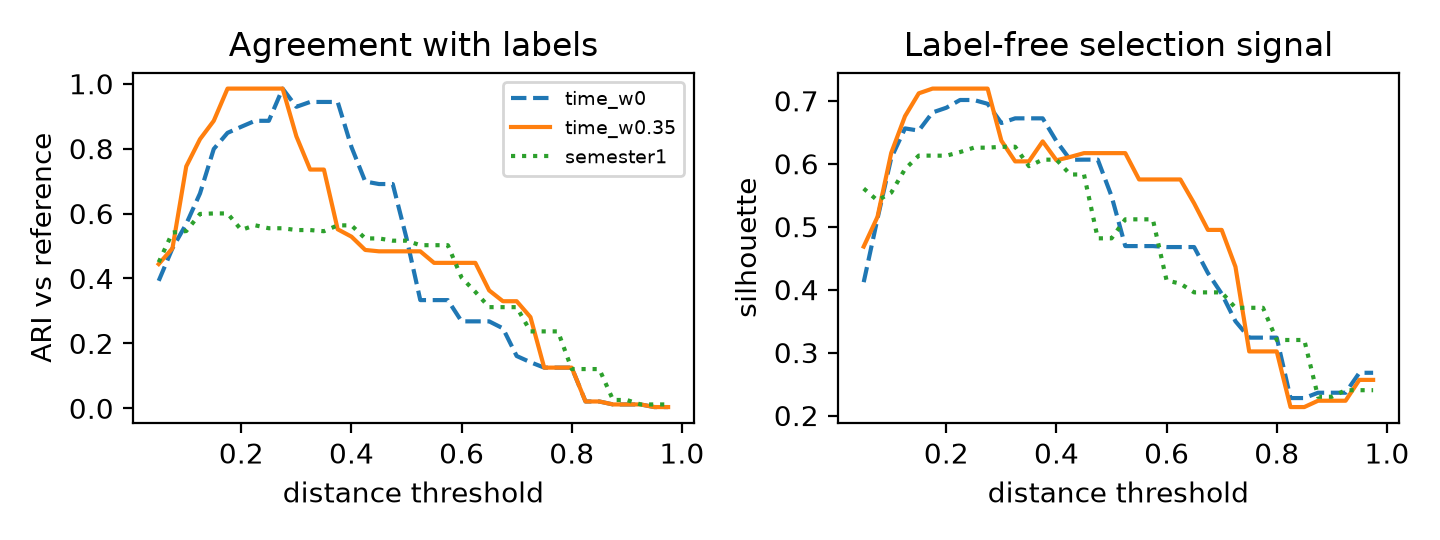
\includegraphics[width=0.92\textwidth]{figures/event_threshold_curves.png}
\caption{Event distance threshold on the 55 photographs. Left: agreement with
the folder grouping. Right: the silhouette the selection rule actually sees.
The production rule takes the silhouette peak of the solid curve.}
\label{fig:eventcurves}
\end{figure*}

\subsection{What moves the best shot}
\label{sec:rank-eval}

There is no label for the best photograph of an occasion, and this paper does
not invent one. The question the set can answer is which part of the ranker
changes the choice. Sixteen of the 20 occasions contain at least two
photographs. For each variant we count how many of those 16 change their
winner relative to the production ranker, the mean Kendall $\tau$ between the
two orders, and how often the winner is a detected blink when the same
occasion also contains an eyes-open frame. NIMA scores on this set run from
$3.26$ to $4.88$.

\begin{table}[t]
\caption{Best-shot ranker on 16 occasions with at least two photographs.
Blink picks are winners with eyes-open below $0.45$ in an occasion that had
an eyes-open alternative.}
\label{tab:rank}
\centering
\scriptsize
\begin{tabular}{@{}>{\raggedright\arraybackslash}p{2.55cm}ccc@{}}
\toprule
Variant & Changed & Kendall $\tau$ & Blinks \\
\midrule
No span floors & 4\,/\,16 & 0.66 & 0 \\
No blink constraint & 3\,/\,16 & 0.70 & 3 \\
Semester~1 rule & 8\,/\,16 & 0.32 & 3 \\
NIMA alone & 12\,/\,16 & $-0.15$ & 4 \\
Without centrality & 4\,/\,16 & 0.64 & 0 \\
Without sharpness & 4\,/\,16 & 0.68 & 0 \\
Without NIMA & 1\,/\,16 & 0.94 & 0 \\
\bottomrule
\end{tabular}
\end{table}

Table~\ref{tab:rank} separates three claims. The blink constraint is not
cosmetic: without it, 3 of the 16 winners are closed-eye frames that had an
open-eye alternative, and the Semester~1 rule, which also lacks the floors,
does the same. An aesthetic score on its own is not a curator. It disagrees
with the full ranker on 12 of 16 winners and agrees with the production order
worse than a reversed ranking. Centrality and sharpness each move 4 winners;
removing NIMA moves 1, and removing face size, detection confidence, pose or
the eyes-open \emph{weight} moves none. The weight can be inert while the
constraint is not. Perturbing any single weight by $\pm 20\%$ changes no winner.

\subsection{A human keep-one-photo study}
\label{sec:pref-eval}

Thirteen people finished a keep-one-photo task on 16 occasions from the same
private collection. Each question showed two, three or four photographs from
one occasion and asked which single photograph they would keep. Twelve
questions updated the ranker: eight, then four more after the held-out block.
Two of those occasions were shown a second time and were not used as updates.
Four occasions were held out and were scored only after every training update.
A pick that differed from the photograph Lumina displayed first was one
step~\eqref{eq:sgd}, one pass, with a separate weight vector for each person.
People are not pooled.

On the two repeated occasions, 16 of 26 second answers matched that person's
first answer, against about 10 if the second answer ignored the first. Seven
of the ten changes moved to a photograph Lumina had ranked lower. People also
disagree with each other. Table~\ref{tab:pref} places every kept photograph in
the displayed order. Rank 1 scores 1 and last place scores 0, so chance is
$0.50$ at every length. The 234 answers score $0.53$. Almost all of that gain
is the top photograph (93 against 84.5). It is not uniform: two-photo questions
carry it, three-photo questions are half the answers and sit at $0.48$, and
four-photo questions are only slightly above chance on the top photograph.

\begin{table}[t]
\caption{Where the kept photograph sits in Lumina's displayed order.
The $0$--$1$ score maps rank 1 to 1 and last place to 0. Chance is a uniform
pick among the photographs on that question. Lower mean rank is closer to the
photograph Lumina showed first. Thirteen finished sittings, 18 questions.}
\label{tab:pref}
\centering
\scriptsize
\resizebox{\columnwidth}{!}{%
\begin{tabular}{@{}lrrrrrrr@{}}
\toprule
& & \multicolumn{2}{c}{Mean rank} & \multicolumn{2}{c}{Score} & \multicolumn{2}{c}{Top-1} \\
\cmidrule(lr){3-4} \cmidrule(lr){5-6} \cmidrule(lr){7-8}
Photos & Picks & Lumina & Chance & Lumina & Chance & Lumina & Chance \\
\midrule
2 & 65 & 1.43 & 1.50 & 0.57 & 0.50 & 37 & 32.5 \\
3 & 117 & 2.04 & 2.00 & 0.48 & 0.50 & 41 & 39 \\
4 & 52 & 2.25 & 2.50 & 0.58 & 0.50 & 15 & 13 \\
All & 234 & 1.92 & 1.97 & 0.53 & 0.50 & 93 & 84.5 \\
\bottomrule
\end{tabular}}
\end{table}

One learning pass does not beat leaving the weights alone. On the 52 held-out
answers the original first photograph matches 26 and the first photograph
after that person's updates matches 24. Three people gain a match and three
lose matches. The other seven keep the same count.

Three conclusions follow. Preference is inconsistent and it varies: a fixed
order cannot match both showings when a person changes, and the thirteen people
do not share one taste, so their sittings stay separate. A score of $0.53$
against $0.50$ is already evidence that the signals are not noise. It is not
a reason to keep a single best picture and delete the rest. A deletion has to
show its reason, or a close call will not be trusted. The seven weights are
also incomplete. On one three-photograph occasion every tester kept the frame
Lumina ranked last: the wide portrait with the whole party, not the tighter
views of three people that scored higher. That is sentimental value in
capturing everybody who was there. Retuning sharpness or NIMA cannot add it.

\section{Discussion}
\label{sec:discuss}

Zero cannot-link merges do not mean the cast is correct. There are no identity
labels, so Section~\ref{sec:id-eval} says nothing about the same person split
apart, and a high $\alpha$ can still trust a wrong ArcFace vector. The event
result is one distance matrix and one person's grouping of 20 occasions.
Twenty-three photographs have no EXIF time, and time cannot split identical
scenes once the threshold exceeds $0.35$. The ranker still has two internal
mismatches: per-person face signals, other than eyes, drop the floors of
Table~\ref{tab:weights}, and MMR can open on a blink because it reads $S$
rather than the constrained order. The retouch guard misses a changed
background or a face the detector never saw.

Further work follows the keep-one study. Repeat more than two occasions, and
keep one weight vector per person, so inconsistency is measured rather than
averaged away. Stop treating one best picture as the curation: several frames
can remain, and a frame set aside should show which signal caused it. The
application's Cleanup view is a first step: it labels each frame it sets aside
as a duplicate, a blink or a blur, and deletes only when the user confirms. Extend
the seven weights. The first candidate is how many of the occasion's people
are in the frame, which is the group-portrait case above, not a larger NIMA
weight. A public album with identity labels, a second grouping of the
occasions, and Recall@$K$ for CLIP search would strengthen the other claims.
They do not replace that measurement.

\section{Conclusion}

On this collection the fused clustering makes no cannot-link merge, the
label-free event threshold matches the best labelled threshold, and the blink
constraint is what keeps closed eyes out of the winners. Thirteen people put the
displayed order only slightly above a random pick. Their preferences vary, a
single keeper is too aggressive unless the deletion says why, and the seven
weights do not yet count the value of having everybody in the frame.

\section*{Acknowledgment}
Ong Qing Quan integrated the baseline pipeline and the web application, and
carried the Semester~2 model improvements and the side models. Agustinus
Benyamin Prasetyo designed the original Semester~1 model, the evaluation and
the human study. An AI coding assistant was used to implement parts of the
software and to draft this paper from the codebase, the Semester~1 report and
the experiment logs. The authors remain responsible for the text.

\balance
\begin{thebibliography}{00}

\bibitem{platt2003phototoc}
J.~C. Platt, M.~Czerwinski, and B.~A. Field,
``PhotoTOC: Automatic clustering for browsing personal photographs,''
in \emph{Proc.\ Joint Conf.\ 4th Int.\ Conf.\ Information, Communications
and Signal Processing and 4th Pacific Rim Conf.\ Multimedia},
2003, doi: 10.1109/ICICS.2003.1292402.

\bibitem{deng2019arcface}
J.~Deng, J.~Guo, N.~Xue, and S.~Zafeiriou,
``ArcFace: Additive angular margin loss for deep face recognition,''
in \emph{Proc.\ IEEE/CVF Conf.\ Computer Vision and Pattern Recognition (CVPR)},
2019, pp.~4690--4699.

\bibitem{insightface}
J.~Guo and others,
``InsightFace: 2D and 3D face analysis project,''
\url{https://github.com/deepinsight/insightface}, accessed 2026.

\bibitem{zhou2019osnet}
K.~Zhou, Y.~Yang, A.~Cavallaro, and T.~Xiang,
``Omni-scale feature learning for person re-identification,''
in \emph{Proc.\ IEEE/CVF Int.\ Conf.\ Computer Vision (ICCV)},
2019, pp.~3702--3712.

\bibitem{jocher2023yolov8}
G.~Jocher, A.~Chaurasia, and J.~Qiu,
``Ultralytics YOLOv8,''
\url{https://github.com/ultralytics/ultralytics}, 2023.

\bibitem{mcinnes2017hdbscan}
L.~McInnes, J.~Healy, and S.~Astels,
``hdbscan: Hierarchical density based clustering,''
\emph{J.\ Open Source Software}, vol.~2, no.~11, p.~205, 2017.

\bibitem{talebi2018nima}
H.~Talebi and P.~Milanfar,
``NIMA: Neural image assessment,''
\emph{IEEE Trans.\ Image Process.}, vol.~27, no.~8, pp.~3998--4011, 2018.

\bibitem{bradley1952rank}
R.~A. Bradley and M.~E. Terry,
``Rank analysis of incomplete block designs: I. The method of paired comparisons,''
\emph{Biometrika}, vol.~39, no.~3/4, pp.~324--345, 1952.

\bibitem{oquab2024dinov2}
M.~Oquab \emph{et al.},
``DINOv2: Learning robust visual features without supervision,''
\emph{Trans.\ Machine Learning Research}, 2024.

\bibitem{simeoni2025dinov3}
O.~Sim\'eoni \emph{et al.},
``\mbox{DINOv3},''
arXiv:2508.10104, 2025.

\bibitem{radford2021clip}
A.~Radford \emph{et al.},
``Learning transferable visual models from natural language supervision,''
in \emph{Proc.\ Int.\ Conf.\ Machine Learning (ICML)}, 2021, pp.~8748--8763.

\bibitem{li2022blip}
J.~Li, D.~Li, C.~Xiong, and S.~Hoi,
``BLIP: Bootstrapping language-image pre-training for unified vision-language understanding and generation,''
in \emph{Proc.\ Int.\ Conf.\ Machine Learning (ICML)}, 2022, pp.~12888--12900.

\bibitem{murray2012ava}
N.~Murray, L.~Marchesotti, and F.~Perronnin,
``AVA: A large-scale database for aesthetic visual analysis,''
in \emph{Proc.\ IEEE Conf.\ Computer Vision and Pattern Recognition (CVPR)},
2012, pp.~2408--2415.

\bibitem{carbonell1998mmr}
J.~Carbonell and J.~Goldstein,
``The use of MMR, diversity-based reranking for reordering documents and producing summaries,''
in \emph{Proc.\ 21st Int.\ ACM SIGIR Conf.\ Research and Development in Information Retrieval},
1998, pp.~335--336.

\bibitem{rousseeuw1987silhouettes}
P.~J. Rousseeuw,
``Silhouettes: A graphical aid to the interpretation and validation of cluster analysis,''
\emph{J.\ Computational and Applied Mathematics}, vol.~20, pp.~53--65, 1987.

\bibitem{pedregosa2011sklearn}
F.~Pedregosa \emph{et al.},
``Scikit-learn: Machine learning in Python,''
\emph{J.\ Machine Learning Research}, vol.~12, pp.~2825--2830, 2011.

\bibitem{soukupova2016eye}
T.~Soukupov\'a and J.~\v{C}ech,
``Real-time eye blink detection using facial landmarks,''
in \emph{Proc.\ Computer Vision Winter Workshop (CVWW)}, 2016.

\bibitem{lugaresi2019mediapipe}
C.~Lugaresi \emph{et al.},
``MediaPipe: A framework for building perception pipelines,''
arXiv:1906.08172, 2019.

\bibitem{hubert1985comparing}
L.~Hubert and P.~Arabie,
``Comparing partitions,''
\emph{J.\ Classification}, vol.~2, no.~1, pp.~193--218, 1985.

\end{thebibliography}

\end{document}
